\documentclass[11pt,a4paper]{article}
\usepackage[utf8]{inputenc}
\usepackage[T1]{fontenc}
\usepackage[spanish,es-noshorthands]{babel}
\usepackage[margin=2.1cm]{geometry}
\usepackage{amsmath,amssymb}
\usepackage{graphicx}
\usepackage{booktabs}
\usepackage{xcolor}
\usepackage{pdflscape}
\usepackage[colorlinks=true,linkcolor=blue!50!black,urlcolor=blue!50!black]{hyperref}
\setlength{\parskip}{4pt}
\setlength{\parindent}{0pt}
\newcommand{\dd}{\mathrm{d}}
\title{Dinámica de la pata del Segway por Lagrange\\
\large Coordenada generalizada \(\theta\). Tres casos: banco, robot parado y robot en el aire}
\author{Proyecto Segway con patas -- Robótica II, UNCUYO}
\date{\today}

\begin{document}
\maketitle

Cada pata es una cuatro barras \(ABCD\) con la bancada \(AB\) rígida con la cabina. El servo en \(A\) gira la
manivela \(AD\); el acoplador \(C\)--\(D\)--\(P\) lleva el eje de la rueda \(P\), que sube y baja casi en
vertical. El mecanismo tiene un solo grado de libertad, \(\theta\).

Lo que cambia de una situación a otra no es el mecanismo sino \emph{qué está quieto}. En un banco de pruebas,
con la cabina amurada, el servo mueve la rueda. Con el robot parado, la rueda apoya en el piso y el servo
mueve la cabina, que pesa casi cuatro veces más. En el aire no hay nada quieto. Son tres dinámicas distintas con
la misma geometría, y se obtienen todas de una sola ecuación cambiando un único vector.

\section{Notación y parámetros}

El dibujo del mecanismo (\texttt{fig\_dinamica.png}) está en la página siguiente. Ejes: origen en \(A\), \(x\)
hacia la derecha del dibujo (hacia atrás del robot), \(y\) hacia arriba. Los ángulos absolutos se miden desde
\(+x\) en sentido antihorario.

\begin{center}\small\setlength{\tabcolsep}{4pt}
\begin{tabular}{l p{7.9cm} l}
\toprule
Símbolo & Qué es & Valor \\
\midrule
\(AB,\;AD,\;BC,\;CD,\;DP\) & largos de las barras & 80, 112, 108, 40.8, 112 mm \\
\(45^\circ\) & inclinación de la bancada \(AB\) respecto de la horizontal & \\
\(\delta\) & ángulo del acoplador en \(D\), de \(D\!\to\!C\) a \(D\!\to\!P\) & \(164^\circ\) \\
\(R_w\) & radio de la rueda & 33 mm \\
\(\theta\) & \textbf{coordenada generalizada}: ángulo de \(AD\) bajo la horizontal, positivo horario & \(10^\circ\) plegada, \(40^\circ\) estirada \\
\(\beta_1,\;\beta_2,\;\beta=\beta_1+\beta_2\) & ángulos en \(B\): \(\angle ABD\), \(\angle DBC\), \(\angle ABC\) & \\
\(\alpha_1,\;\alpha_2\) & ángulos en \(D\): \(\angle ADB\), \(\angle BDC\) & \\
\(\psi\) & giro del acoplador: dirección de \(D\!\to\!C\) & \\
\(d_Q,\;\varepsilon_Q\) & un punto \(Q\) del acoplador: distancia desde \(D\) y ángulo desde \(D\!\to\!C\) & \\
\(m_{AD},\;m_{BC},\;m_{CDP}\) & masa de cada pieza de la pata & 23.2, 5.6, 15.6 g \\
\(m_P\) & rueda + motor colgados de \(P\) & 30 + 152 = 182 g \\
\(m_c\) & \textbf{cabina}: cabeza, tapa, servos, batería, electrónica, tornillería & 667 g \\
\(m\) & masa del robot, \(m=m_c+n\,(m_{AD}+m_{BC}+m_{CDP}+m_P)\) & 1120 g \\
\(n\) & patas iguales, movidas a la vez por sus \(n\) servos & 2 \\
\(AG,\;BG\) & distancia de \(A\) a \(G_{AD}\) y de \(B\) a \(G_{BC}\) & \(0.428\,AD\), \(0.5\,BC\) \\
\(d_G,\;\varepsilon_G\) & posición de \(G_{CDP}\) desde \(D\) (sobre la recta \(D\!\to\!P\)) & \(0.3145\,DP\), \(\delta\) \\
\(I_{AD},I_{BC},I_{CDP}\) & inercia de cada pieza respecto de \emph{su propio} centro de masa & 3.6, 0.9, 3.3 \(\cdot10^{-5}\) kg\,m\(^2\) \\
\(\tau\) & par de un servo sobre su manivela, positivo en el sentido en que crece \(\theta\) & \(\le 40\) kg\,cm \\
\(N\) & reacción del piso sobre una rueda, hacia arriba & \\
\(b\) & fricción viscosa en el eje del servo & \\
\bottomrule
\end{tabular}
\end{center}

Todo se escribe \textbf{por servo}: las \(n\) patas se mueven juntas, así que la energía del robot se divide
entre los \(n\) servos y por eso la cabina aparece como \(m_c/n\). El ángulo interior en \(A\) entre \(AB\) y
\(AD\) es \(\theta+45^\circ\); el ángulo absoluto del servo que usa la cinemática es \(360^\circ-\theta\).
De la cabina solo hace falta la masa, no dónde está su centro de masa, porque no gira: se supone que el
control de equilibrio mantiene la inclinación del robot mientras la pata se mueve. Las masas e inercias de las barras son
las de la primera iteración del CAD escaladas a 80; el motor y el servo, los de sus fichas. Todo se reemplaza pesando. Todos los valores están en la sección 1 de
\texttt{dinamica\_pata.m}.

\begin{landscape}
\vspace*{\fill}
\begin{center}

\includegraphics[width=\linewidth]{fig_dinamica.png}
\end{center}
\vspace*{\fill}
\end{landscape}

\section{Geometría}

\textbf{Diagonal.} Ley del coseno en \(ABD\), con el ángulo \(\theta+45^\circ\) en \(A\):
\begin{equation}
BD=\sqrt{AB^2+AD^2-2\,AB\,AD\cos(\theta+45^\circ)} .
\label{eq:BD}
\end{equation}

\textbf{Ángulos en \(B\) y en \(D\).} Ley del coseno en los triángulos \(ABD\) y \(BDC\), que comparten \(BD\):
\begin{align}
\beta_1&=\cos^{-1}\!\left(\frac{AD^2-AB^2-BD^2}{-2\,AB\,BD}\right), &
\beta_2&=\cos^{-1}\!\left(\frac{DC^2-BC^2-BD^2}{-2\,BC\,BD}\right), &
\beta&=\beta_1+\beta_2, \label{eq:beta}\\
\alpha_1&=\cos^{-1}\!\left(\frac{AB^2-BD^2-AD^2}{-2\,BD\,AD}\right), &
\alpha_2&=\cos^{-1}\!\left(\frac{BC^2-BD^2-DC^2}{-2\,BD\,DC}\right).&& \label{eq:alfa}
\end{align}
\(\beta\) es el ángulo interior del balancín en \(B\). Las sumas valen en la configuración abierta, con \(D\)
entre \(BA\) y \(BC\), que es la del CAD.

\textbf{Giro del acoplador.} En \(D\), la dirección \(D\!\to\!A\) forma \(180^\circ-\theta\) con \(+x\)
(ángulos alternos internos entre las horizontales por \(A\) y por \(D\)). Girando \(\alpha_1\) en sentido
horario se llega a \(D\!\to\!B\), y \(\alpha_2\) más a \(D\!\to\!C\):
\begin{equation}
\boxed{\;\psi=180^\circ-\theta-\alpha_1-\alpha_2\;}
\label{eq:psi}
\end{equation}
Como \(C\)--\(D\)--\(P\) es una pieza rígida, \(\psi\) es el giro de todo el acoplador, y el lado \(D\!\to\!P\)
apunta en la dirección \(\psi+\delta\).

\textbf{Posiciones.} \(A=(0,0)\), \(B=AB\,(\cos45^\circ,\;\sin45^\circ)\) y
\begin{equation}
D=\bigl(AD\cos\theta,\;-AD\sin\theta\bigr).
\label{eq:D}
\end{equation}
Un punto \(Q\) del acoplador, a distancia \(d_Q\) de \(D\) y a un ángulo \(\varepsilon_Q\) desde \(D\!\to\!C\):
\begin{equation}
Q=\bigl(AD\cos\theta+d_Q\cos(\psi+\varepsilon_Q),\;\;-AD\sin\theta+d_Q\sin(\psi+\varepsilon_Q)\bigr),
\label{eq:Q}
\end{equation}
con \((d_Q,\varepsilon_Q)=(CD,0)\) para \(C\), \((DP,\delta)\) para el eje de la rueda \(P\) y
\((d_G,\varepsilon_G)\) para \(G_{CDP}\). Los otros dos centros de masa giran alrededor de pivotes fijos a la
cabina: \(G_{AD}=AG\,(\cos\theta,\,-\sin\theta)\) y
\(G_{BC}=B+BG\,(\cos(225^\circ+\beta),\,\sin(225^\circ+\beta))\), ya que \(B\!\to\!A\) apunta a \(225^\circ\)
y \(B\!\to\!C\) está \(\beta\) más allá en sentido antihorario. Comprobación del cierre: \(C\) calculado con
\eqref{eq:Q} y \(C=B+BC\,(\cos(225^\circ+\beta),\sin(225^\circ+\beta))\) coinciden para todo \(\theta\).

\section{Velocidades vistas desde la cabina}

Primero se resuelve el mecanismo como si la cabina estuviera quieta. Después, en la sección 4, se le suma el
movimiento de la cabina. Como \(\beta\) y \(\psi\) son funciones de \(\theta\), escribimos
\(\beta'=\dd\beta/\dd\theta\) y \(\psi'=\dd\psi/\dd\theta\).

\textbf{Derivada de la diagonal.} De \eqref{eq:BD}:
\begin{equation}
BD'=\frac{AB\,AD\,\sin(\theta+45^\circ)}{BD}.
\label{eq:dBD}
\end{equation}

\textbf{Derivada de un ángulo respecto de un lado.} Los cuatro ángulos de \eqref{eq:beta}--\eqref{eq:alfa}
dependen de \(\theta\) solo a través de \(BD\). En un triángulo de lados \(p\), \(q\), \(r\), sea \(\alpha\)
el ángulo entre \(p\) y \(q\), y \(\alpha_q\) el ángulo del otro extremo de \(q\), entre \(q\) y \(r\).
Derivando \(\cos\alpha=(p^2+q^2-r^2)/(2pq)\) respecto de \(q\), con \(p\) y \(r\) fijos, y usando
\(p^2=q^2+r^2-2qr\cos\alpha_q\):
\[
-\sin\alpha\,\frac{\dd\alpha}{\dd q}=\frac{q^2+r^2-p^2}{2pq^2}=\frac{r\cos\alpha_q}{pq}.
\]
Con el teorema del seno, \(r/\sin\alpha=p/\sin\alpha_q\), queda
\begin{equation}
\frac{\dd\alpha}{\dd q}=-\frac{\cot\alpha_q}{q}.
\label{eq:lema}
\end{equation}
Al alargar un lado, el ángulo en un extremo cambia con la cotangente del ángulo en el \emph{otro} extremo.
Aplicado con \(q=BD\):
\begin{equation}
\frac{\dd\beta_1}{\dd BD}=-\frac{\cot\alpha_1}{BD},\quad
\frac{\dd\beta_2}{\dd BD}=-\frac{\cot\alpha_2}{BD},\quad
\frac{\dd\alpha_1}{\dd BD}=-\frac{\cot\beta_1}{BD},\quad
\frac{\dd\alpha_2}{\dd BD}=-\frac{\cot\beta_2}{BD}.
\label{eq:dang}
\end{equation}

\textbf{Relaciones de transmisión.} Regla de la cadena con \eqref{eq:dBD} y \eqref{eq:dang} sobre
\(\beta=\beta_1+\beta_2\) y \(\psi=180^\circ-\theta-\alpha_1-\alpha_2\):
\begin{equation}
\boxed{\;
\begin{aligned}
\beta'(\theta)&=-\bigl(\cot\alpha_1+\cot\alpha_2\bigr)\,\frac{AB\,AD\,\sin(\theta+45^\circ)}{BD^2}\\[2pt]
\psi'(\theta)&=-1+\bigl(\cot\beta_1+\cot\beta_2\bigr)\,\frac{AB\,AD\,\sin(\theta+45^\circ)}{BD^2}
\end{aligned}
\;}
\label{eq:dbeta_dpsi}
\end{equation}
Las velocidades angulares de las tres piezas, medidas desde la cabina y positivas antihorarias, son
\(\omega_{AD}=-\dot\theta\), \(\omega_{BC}=\beta'\dot\theta\) y \(\omega_{CDP}=\psi'\dot\theta\).

\textbf{Coeficientes de velocidad.} Para cada punto \(Q\) del mecanismo se define \(c_Q(\theta)\), su velocidad
vista desde la cabina por unidad de \(\dot\theta\):
\begin{equation}
\mathbf{v}^{\,\text{cabina}}_Q=c_Q(\theta)\,\dot\theta,\qquad c_Q=\frac{\dd Q}{\dd\theta}.
\label{eq:cQ}
\end{equation}
Con \(\mathbf{k}\times(x,y)=(-y,x)\), los tres cuerpos dan:
\begin{align}
\text{manivela } AD:&\quad c_D=-\,\mathbf{k}\times D, \qquad c_{G_{AD}}=-\,\mathbf{k}\times G_{AD}; \label{eq:cAD}\\
\text{balancín } BC:&\quad c_{G_{BC}}=\beta'\,\mathbf{k}\times\bigl(G_{BC}-B\bigr); \label{eq:cBC}\\
\text{acoplador } CDP:&\quad c_Q=c_D+\psi'\,\mathbf{k}\times\bigl(Q-D\bigr) \quad\text{para } Q=C,\,P,\,G_{CDP}. \label{eq:cCDP}
\end{align}
La segunda componente de \(c_P\) es \(y_P'(\theta)\), la velocidad vertical del eje de la rueda respecto de la
cabina. Es negativa en toda la carrera: al crecer \(\theta\) la rueda baja respecto de la cabina.

\begin{landscape}
\vspace*{\fill}
\begin{center}
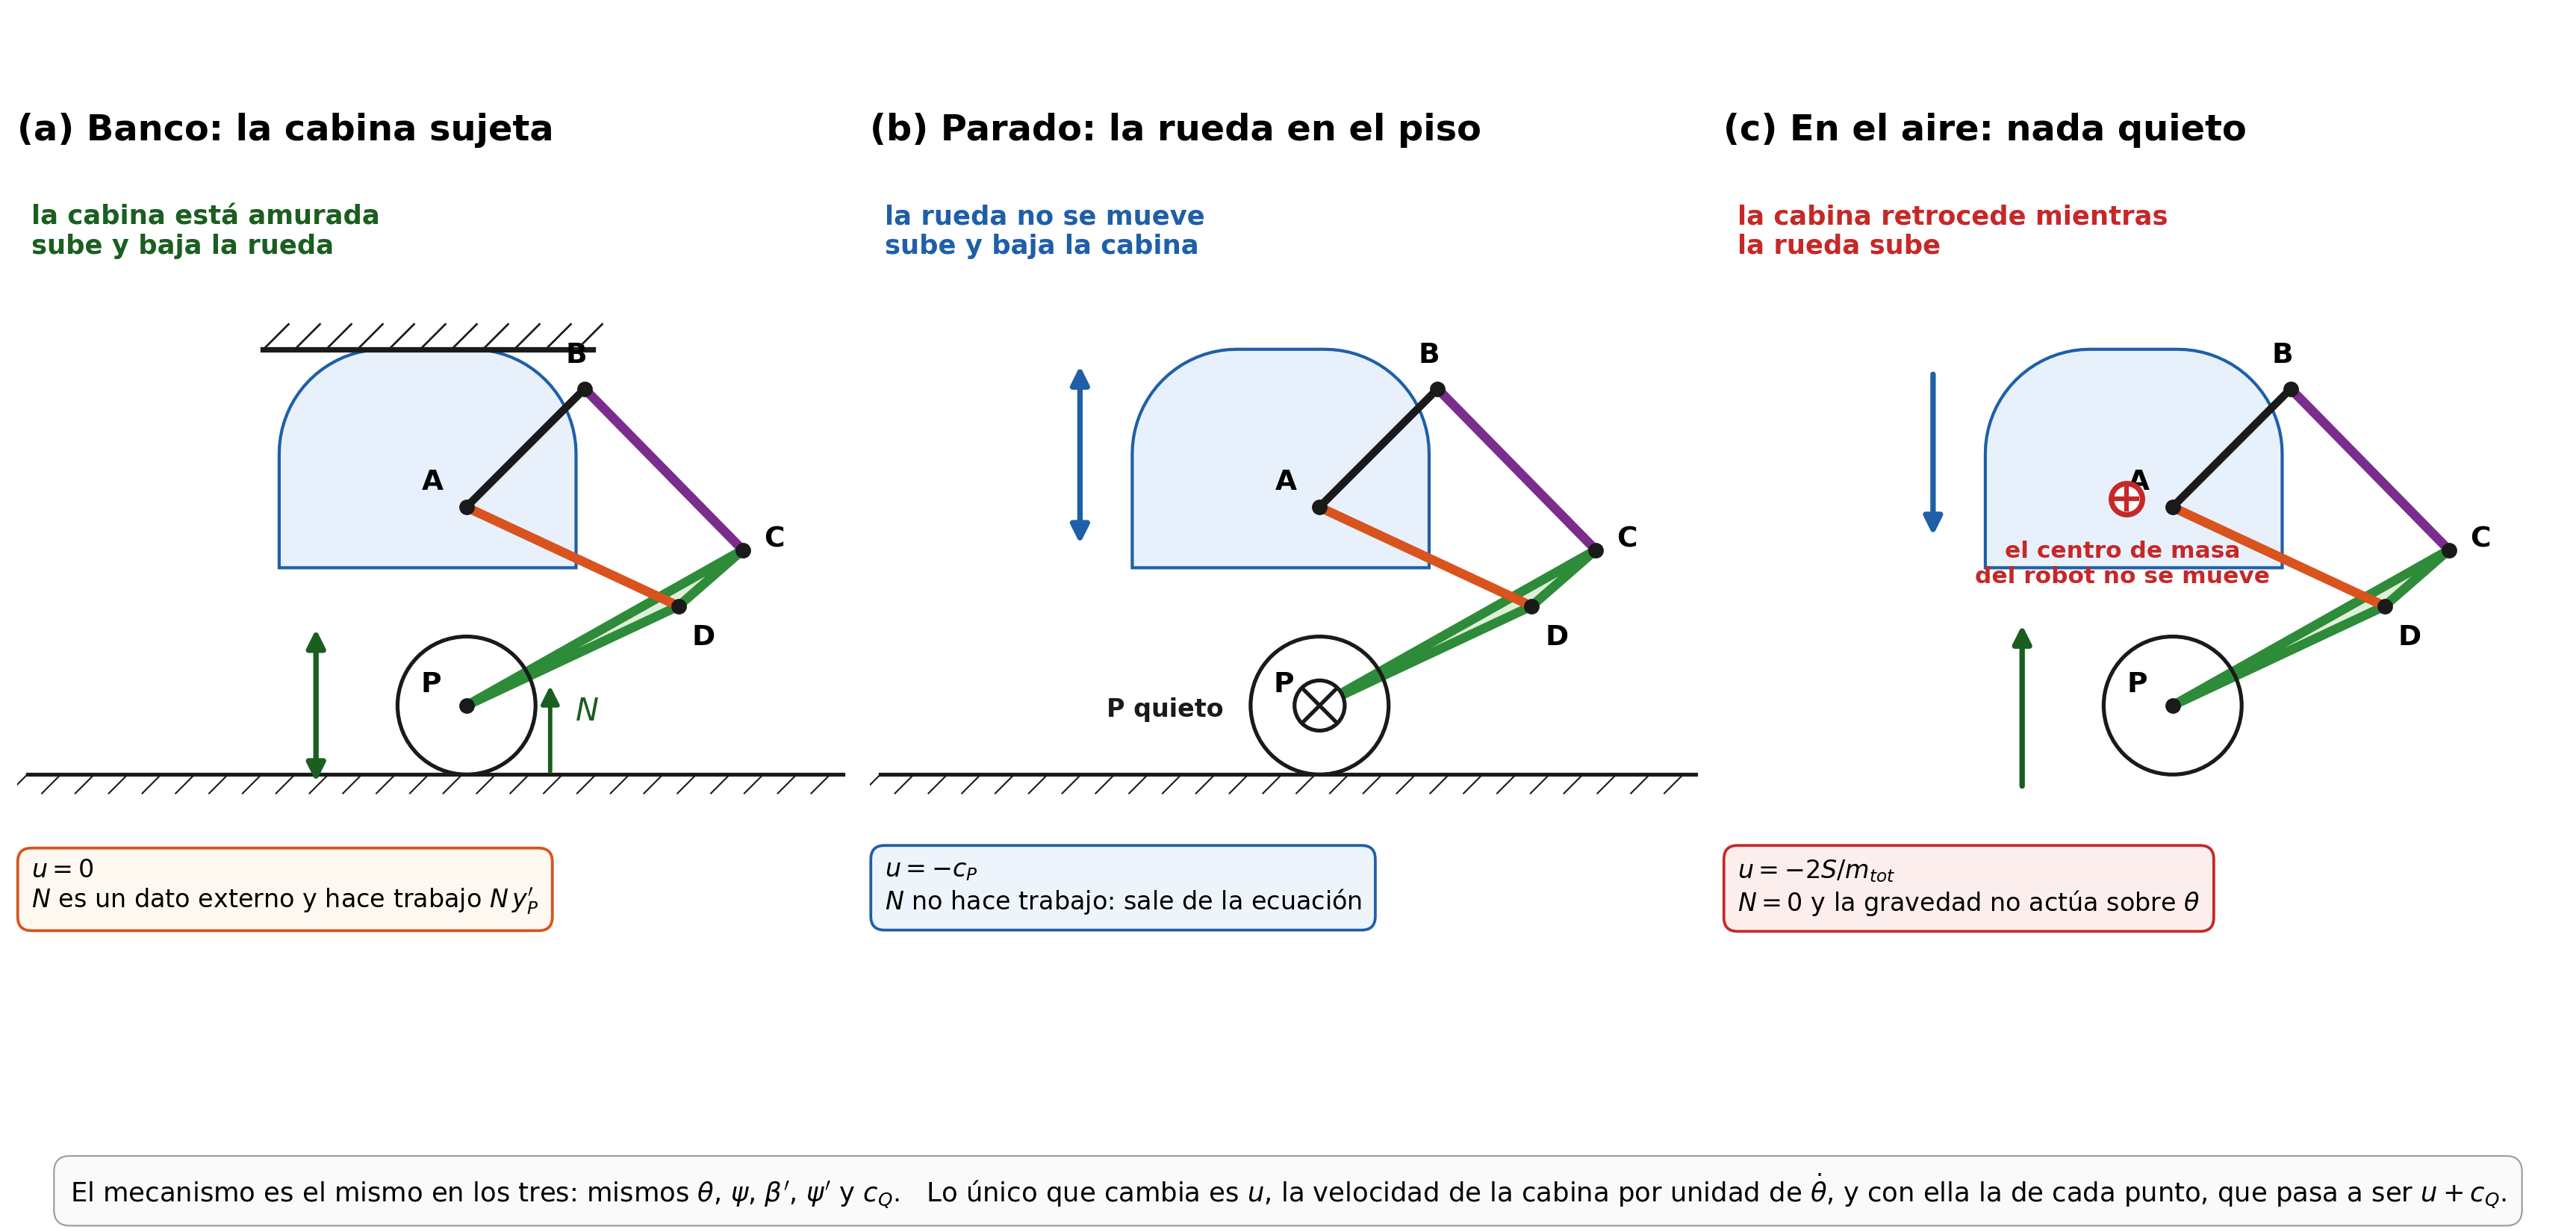
\includegraphics[width=\linewidth]{fig_casos.png}
\end{center}
\vspace*{\fill}
\end{landscape}

\section{Los tres casos: qué está quieto}

La figura de la página anterior muestra los tres. La cabina no gira, solo se traslada. Basta entonces un vector \(u(\theta)\), su velocidad por unidad de
\(\dot\theta\), para pasar del marco de la cabina al del piso. Todo punto de la cabina se mueve con
\(u\,\dot\theta\), y todo punto del mecanismo con
\begin{equation}
\mathbf{v}_Q=\bigl(u+c_Q\bigr)\dot\theta .
\label{eq:vpiso}
\end{equation}

\textbf{(a) Banco.} La cabina está amurada:
\begin{equation}
u=0 .
\label{eq:ubanco}
\end{equation}
La reacción del piso \(N\) es un dato externo y hace trabajo sobre la rueda, que sube y baja.

\textbf{(b) Parado.} La rueda apoya y el eje \(P\) queda a la altura \(R_w\) del piso. Si \(Y_A\) es la altura
de \(A\), la condición de apoyo es \(Y_A+y_P(\theta)=R_w\), de donde \(Y_A=R_w-y_P(\theta)\): la altura de la
cabina es una función de \(\theta\) que ya teníamos. Derivando, y suponiendo que la rueda queda quieta,
\begin{equation}
u=-c_P .
\label{eq:uparado}
\end{equation}
Ahora \(N\) no hace trabajo, porque el punto de contacto no se mueve, y desaparece de la ecuación. El peso de
la cabina, que en el caso (a) entraba disfrazado dentro de \(N\), pasa a estar donde corresponde, en la
energía potencial.

\textbf{(c) En el aire.} Nada está quieto y no hay fuerzas externas salvo la gravedad, así que el centro de
masa del robot no se mueve respecto de la caída libre. El momento lineal relativo es nulo:
\(m_c\,u+n\sum_j m_j\,(u+c_j)=0\), sumando sobre las piezas \(j\) de una pata. Con
\(S=\sum_j m_j c_j\) queda
\begin{equation}
u=-\,\frac{n\,S}{m},\qquad S=m_{AD}c_{G_{AD}}+m_{BC}c_{G_{BC}}+m_{CDP}c_{G_{CDP}}+m_P\,c_P .
\label{eq:uaire}
\end{equation}

\section{Energía cinética}

Cada pieza contribuye con la traslación de su centro de masa más su giro propio (König). Las velocidades son
las de \eqref{eq:vpiso}, y las angulares no dependen del caso porque la cabina no gira. Dividiendo la energía
del robot entre los \(n\) servos, \(K=\tfrac12\,I_{eq}(\theta)\,\dot\theta^2\) con
\begin{equation}
\boxed{\;
\begin{aligned}
I_{eq}(\theta)={}&\underbrace{I_{AD}+I_{BC}\,\beta'^2+I_{CDP}\,\psi'^2}_{\text{giro propio de las tres piezas}}
\;+\;\underbrace{\frac{m_c}{n}\,\bigl|u\bigr|^2}_{\text{cabina}}\\[2pt]
&+\;m_{AD}\bigl|u+c_{G_{AD}}\bigr|^2+m_{BC}\bigl|u+c_{G_{BC}}\bigr|^2
+m_{CDP}\bigl|u+c_{G_{CDP}}\bigr|^2+m_P\bigl|u+c_P\bigr|^2
\end{aligned}
\;}
\label{eq:Ieq}
\end{equation}
Una sola fórmula para los tres casos: se reemplaza \(u\) por \eqref{eq:ubanco}, \eqref{eq:uparado} o
\eqref{eq:uaire}. Vale la pena mirar qué queda en cada uno.

\begin{center}\small
\begin{tabular}{lll}
\toprule
Caso & Término dominante & Por qué \\
\midrule
Banco, \(u=0\) & \(m_P\,|c_P|^2\) & el servo acelera la rueda y el motor, 182 g \\
Parado, \(u=-c_P\) & \(\dfrac{m_c}{n}\,|c_P|^2\) & la rueda está quieta y el servo acelera media cabina, 334 g \\
En el aire & ninguno domina & la cabina retrocede y el conjunto se reparte el movimiento \\
\bottomrule
\end{tabular}
\end{center}

Parado, el término de \(m_P\) desaparece por completo (la rueda no se traslada) y lo reemplaza uno con casi
el doble de masa. Ese es el motivo de que la inercia vista por el servo sea 1.85 veces mayor que en el banco.

\section{Energía potencial}

Solo gravedad. Con \(y\) hacia arriba y las alturas medidas desde el piso,
\begin{equation}
V(\theta)=g\left[\frac{m_c}{n}\,Y_A+m_{AD}\,y_{G_{AD}}+m_{BC}\,y_{G_{BC}}+m_{CDP}\,y_{G_{CDP}}+m_P\,y_P\right],
\label{eq:V}
\end{equation}
y como la velocidad vertical de cada punto por unidad de \(\dot\theta\) es la segunda componente de
\(u+c_Q\), la derivada sale directamente:
\begin{equation}
\boxed{\;
\begin{aligned}
V'(\theta)=g\Bigl[&\frac{m_c}{n}\,u_y+m_{AD}\bigl(u_y+c_{G_{AD},y}\bigr)+m_{BC}\bigl(u_y+c_{G_{BC},y}\bigr)\\
&+m_{CDP}\bigl(u_y+c_{G_{CDP},y}\bigr)+m_P\bigl(u_y+c_{P,y}\bigr)\Bigr]
\end{aligned}
\;}
\label{eq:dV}
\end{equation}
En el caso del aire, \eqref{eq:dV} con \(u\) de \eqref{eq:uaire} da exactamente cero: en caída libre la
gravedad no actúa sobre \(\theta\), y el servo solo pelea contra la inercia. Es una buena comprobación de que
las tres fórmulas son consistentes.

\section{Fuerzas generalizadas}

Entran por su trabajo virtual, \(\delta W=Q_\theta\,\delta\theta\): el par del servo actúa directamente sobre
\(\theta\); la fricción del eje da \(-b\,\dot\theta\); la reacción del piso \(N\) trabaja sobre el
desplazamiento vertical de la rueda, que por \eqref{eq:vpiso} es \(w_P\,\delta\theta\) con
\(w_P=u_y+c_{P,y}\):
\begin{equation}
Q_\theta=\tau-b\,\dot\theta+N\,w_P,\qquad
w_P=\begin{cases} y_P'(\theta) & \text{banco}\\ 0 & \text{parado}\\ - & \text{en el aire }(N=0)\end{cases}
\label{eq:Qtheta}
\end{equation}

\section{Ecuación de movimiento}

Con \(L=K-V=\tfrac12 I_{eq}(\theta)\dot\theta^2-V(\theta)\), la ecuación de Lagrange
\(\dfrac{\dd}{\dd t}\dfrac{\partial L}{\partial\dot\theta}-\dfrac{\partial L}{\partial\theta}=Q_\theta\) da
\begin{equation}
\boxed{\;
I_{eq}(\theta)\,\ddot\theta+\tfrac12\,I_{eq}'(\theta)\,\dot\theta^2+V'(\theta)=\tau-b\,\dot\theta+N\,w_P(\theta)
\;}
\label{eq:final}
\end{equation}
con \(I_{eq}\) de \eqref{eq:Ieq}, \(V'\) de \eqref{eq:dV} y \(w_P\) de \eqref{eq:Qtheta}. El término
\(\tfrac12 I_{eq}'\dot\theta^2\) es el propio de un mecanismo con inercia variable; \(I_{eq}'\) se calcula
numéricamente.

\textbf{Par estático.} Con la pata quieta,
\begin{equation}
\tau_{est}(\theta)=V'(\theta)-N\,w_P(\theta).
\label{eq:tau_est}
\end{equation}
Los casos (a) y (b) dan el mismo número si en el banco se carga la rueda con \(N=m\,g/n\), el peso que
soporta cada pata del robot parado. No es casualidad: el trabajo virtual es el mismo se mire desde donde se
mire, y \(N\) ya incluye el peso de la cabina. Por eso el dimensionamiento del servo no cambia entre los dos
casos; lo que cambia es solo la parte dinámica.

\textbf{Normal en el piso.} Parado, \(N\) no aparece en \eqref{eq:final} pero conviene calcularla para saber
si la rueda sigue apoyada. Si \(Y'_{cm}(\theta)\) es la velocidad vertical del centro de masa del robot por
unidad de \(\dot\theta\), que sale de \eqref{eq:dV} como \(Y'_{cm}=n\,V'/(m\,g)\), entonces
\begin{equation}
N=\frac{m}{n}\Bigl[g+Y'_{cm}\,\ddot\theta+Y''_{cm}\,\dot\theta^2\Bigr].
\label{eq:N}
\end{equation}
Si \(N\) llega a cero el robot despega, y a partir de ahí vale el caso (c).

\textbf{Para simular.} En forma de estado, con \(x=(\theta,\dot\theta)\):
\begin{equation}
\ddot\theta=\frac{\tau-b\,\dot\theta+N\,w_P-\tfrac12 I_{eq}'\,\dot\theta^2-V'}{I_{eq}} .
\label{eq:estado}
\end{equation}

\section{Valores numéricos}

Con los parámetros de la tabla, \(n=2\), y \(N=m\,g/2=5.49\) N para el par estático del banco:

\begin{center}\small
\begin{tabular}{lrrr}
\toprule
 & \(\theta=10^\circ\) (plegada) & \(\theta=25^\circ\) & \(\theta=40^\circ\) (estirada) \\
\midrule
Altura de la cabina \(h=R_w-y_P\) [mm] & 70.2 & 127.9 & 177.2 \\
\(\beta'\), \(\psi'\) [rad/rad] & \(-0.703\), \(1.260\) & \(-0.950\), \(0.964\) & \(-1.161\), \(1.120\) \\
\(y_P'\) [mm/rad] & \(-250\) & \(-199\) & \(-182\) \\
\midrule
\(I_{eq}\) banco [g\,m\(^2\)] & 11.86 & 7.66 & 6.43 \\
\(I_{eq}\) parado [g\,m\(^2\)] & \textbf{22.24} & \textbf{14.13} & \textbf{11.92} \\
\(I_{eq}\) en el aire [g\,m\(^2\)] & 7.56 & 4.86 & 4.13 \\
parado / banco & 1.87 & 1.84 & 1.85 \\
\midrule
\(\tau_{est}\) banco con \(N=m g/2\) [kg\,cm] & 9.06 & 7.20 & 6.58 \\
\(\tau_{est}\) parado [kg\,cm] & 9.06 & 7.20 & 6.58 \\
\(\tau_{est}\) en el aire [kg\,cm] & 0 & 0 & 0 \\
\bottomrule
\end{tabular}
\end{center}

Lecturas. El par estático es idéntico en los dos primeros casos, como anticipa \eqref{eq:tau_est}, y nulo en
el tercero, como anticipa \eqref{eq:dV}. Parado, cada servo sostiene hasta 9.1 kg\,cm contra los 40 kg\,cm
nominales del servo elegido. La inercia del caso parado es 1.85 veces la del banco, así que un modelo hecho con la
cabina fija subestima casi al doble el par de aceleración: da igual en maniobras lentas y no da igual al
plegarse rápido o al aterrizar.

\textbf{Agacharse y pararse} (sección 3 de \texttt{dinamica\_pata.m}): de \(40^\circ\) a \(10^\circ\) y de
vuelta, en 0.6 s cada tramo, con el robot de pie. El par pico llega a 11.7 kg\,cm, dentro de los 40
disponibles, y la normal por rueda baja de 5.49 N a 1.92 N en el tramo de bajada. El robot no despega, pero
queda en poco más de una tercera parte de su peso de apoyo: en una maniobra más rápida despegaría, y ahí hay que
pasar al caso (c).

\section{Caída de un escalón}

El robot rueda, sale de un escalón de altura \(h\) y cae. Es la maniobra que más exige al servo, porque la
pata tiene que frenar a toda la cabina en la carrera que le queda. Se resuelve en tres fases, con el caso
(c) para la caída y el caso (b) a partir del impacto.

Hipótesis: el eje de la rueda baja exactamente \(h\); la pata llega al piso estirada (\(\theta=40^\circ\)),
que es lo que deja toda la carrera disponible para absorber; las dos ruedas tocan a la vez; el piso y el
neumático son rígidos durante el impacto.

\textbf{Fase 1: caída libre.} Con la rueda en el aire vale el caso (c), y ahí la gravedad no actúa sobre
\(\theta\): el servo solo tiene que mantener la postura. La rueda llega al piso con
\begin{equation}
v=\sqrt{2\,g\,h},\qquad t_{ca\text{í}da}=\frac{v}{g}.
\label{eq:caida}
\end{equation}

\textbf{Fase 2: impacto.} Al tocar, la rueda se detiene de golpe pero la cabina sigue bajando, y eso arrastra
a \(\theta\). Es un problema impulsivo, y para plantearlo hay que soltar la restricción por un instante: se
usan dos coordenadas, la altura \(Y_A\) de la cabina y \(\theta\). La energía cinética por servo en esas
coordenadas da la matriz de masa
\begin{equation}
M=\begin{pmatrix} m/n & S_y \\ S_y & I_{eq}^{\,\text{banco}}\end{pmatrix},
\qquad S_y=\sum_j m_j\,c_{j,y},
\label{eq:Mimpacto}
\end{equation}
donde la suma recorre las piezas de una pata. El impulso \(\hat J\) del piso es vertical y actúa sobre el
punto de contacto, cuya altura es \(Y_A+y_P(\theta)-R_w\), así que se reparte como \((1,\;y_P')\):
\begin{equation}
M\bigl(\dot q^{+}-\dot q^{-}\bigr)=\hat J\begin{pmatrix}1\\ y_P'\end{pmatrix},
\qquad \dot q^{-}=\begin{pmatrix}-v\\ 0\end{pmatrix},
\qquad \dot q^{+}=\begin{pmatrix}-y_P'\,\dot\theta^{+}\\ \dot\theta^{+}\end{pmatrix},
\label{eq:impulso}
\end{equation}
donde \(\dot q^{+}\) ya cumple la condición de apoyo. Eliminando \(\hat J\) entre las dos filas:
\begin{equation}
\boxed{\;
\dot\theta^{+}=\frac{v\left(\dfrac{m}{n}\,y_P'-S_y\right)}{I_p},
\qquad I_p=I_{eq}^{\,\text{banco}}-2\,S_y\,y_P'+\frac{m}{n}\,y_P'^{\,2}
\;}
\label{eq:dthimp}
\end{equation}
\(I_p\) es la inercia con la rueda apoyada, es decir el \(I_{eq}\) del caso (b). Como \(y_P'<0\),
\(\dot\theta^{+}\) es negativa: la pata arranca a plegarse sola. La energía por servo pasa de
\(K^{-}=\tfrac12\,(m/n)\,v^2\) a
\begin{equation}
K^{+}=\tfrac12\,I_p\,\bigl(\dot\theta^{+}\bigr)^2,
\label{eq:Kimp}
\end{equation}
y la diferencia se pierde en el golpe: es el movimiento de la rueda y el motor, que se detienen de golpe.

\textbf{Fase 3: absorción.} A partir de acá vale el caso (b). La pata se pliega de \(\theta_{land}\) hacia el
tope \(\theta_{tope}\) y el servo tiene que frenarla. Como el peso de la cabina también empuja hacia el
plegado, el servo debe disipar la energía del golpe \emph{más} la que suma la gravedad en toda la carrera:
\begin{equation}
E_{abs}=K^{+}+\Delta V,\qquad
\Delta V=V(\theta_{land})-V(\theta_{tope})=\int_{\theta_{tope}}^{\theta_{land}}V'(\theta)\,\dd\theta,
\label{eq:Eabs}
\end{equation}
y el par medio que hace falta sobre la carrera \(\Delta\theta=\theta_{land}-\theta_{tope}\) es
\begin{equation}
\boxed{\;\bar\tau=\frac{E_{abs}}{\Delta\theta}=\frac{K^{+}+\Delta V}{\theta_{land}-\theta_{tope}}\;}
\label{eq:taumedio}
\end{equation}
Dando vuelta la cuenta sale el escalón más alto que el servo puede absorber frenando a fondo sin llegar al
tope, de \(\tau_{max}\,\Delta\theta=K^{+}(h_{max})+\Delta V\). Como \(K^{+}\) es proporcional a \(h\),
\begin{equation}
h_{max}=h\;\frac{\tau_{max}\,\Delta\theta-\Delta V}{K^{+}(h)} .
\label{eq:hmax}
\end{equation}

\textbf{Resultados para \(h=18\) cm}, con la pata llegando estirada y los dos servos frenando a fondo:

\begin{center}\small
\begin{tabular}{lrl}
\toprule
 & Valor & \\
\midrule
Tiempo de caída, velocidad al tocar & 192 ms, 1.88 m/s & \eqref{eq:caida} \\
Velocidad de plegado tras el golpe & 10.4 rad/s = 597\(^\circ\)/s & \eqref{eq:dthimp} \\
Energía por servo, antes \(\to\) después del golpe & 0.989 \(\to\) 0.645 J & \eqref{eq:Kimp} \\
Energía que suma la gravedad al plegar, \(\Delta V\) & 0.380 J & \eqref{eq:Eabs} \\
Energía a disipar por servo, \(E_{abs}\) & 1.024 J & \eqref{eq:Eabs} \\
\textbf{Par medio necesario} \(\bar\tau\) & \textbf{1.96 N\,m = 19.9 kg\,cm} & \eqref{eq:taumedio} \\
Par disponible (servo elegido) & 40 kg\,cm & \\
Escalón máximo absorbible \(h_{max}\) & 47 cm & \eqref{eq:hmax} \\
Fuerza contra el piso mientras el servo frena & 23 N por rueda, 4.3 veces la estática & \eqref{eq:N} \\
\bottomrule
\end{tabular}
\end{center}

\textbf{Con 18 cm alcanza, y sobra.} Hacen falta 19.9 kg\,cm contra los 40 del servo: frenando a fondo, la pata
se detiene en 39 ms usando \(11.4^\circ\) de los \(30^\circ\) de carrera, sin llegar al tope. El límite teórico de este
servo es un escalón de 47 cm, aunque mucho antes el problema deja de ser el servo y pasa a ser la estructura:
a 40 kg\,cm el eje del servo ve 93 N durante el frenado (sección 6 de \texttt{dinamica\_pata.m}).

Dos números más que conviene mirar. La pata se pliega a \(597^\circ\)/s, más rápido que la velocidad en vacío
del propio servo, que ronda los \(400^\circ\)/s: en el aterrizaje el servo no manda, lo manda el golpe, y solo
puede frenar. Y el golpe se lleva el 35 por ciento de la energía: es el momento de la rueda y el motor (182 g), que
se detienen de golpe contra el piso. Ese instante, y no el frenado, es el que más carga la estructura: el
neumático recibe unos 144 N (26 veces la carga estática) y el eje del servo, del orden de 460 N.

Ese pico del toque no depende del servo sino de la masa que cuelga de \(P\): con el motor en la rueda (152 de
los 182 g) el golpe se lleva el 35 por ciento de la energía; con el motor en la cabina y transmisión por correa se
llevaría del orden del 10. Es la decisión de diseño que más cambia la carga sobre los pasadores y el neumático.

\section{Alcance}

Los tres casos suponen que la cabina no gira mientras la pata se mueve, es decir que el control de equilibrio
mantiene la inclinación, y que las \(n\) patas se mueven juntas. Con eso alcanza para dimensionar el servo,
para elegir cuán rápido se puede agachar y pararse el robot, para saber cuándo despega y para calcular
qué escalón puede bajar.

Lo que no cubre es el equilibrio en sí: cómo el movimiento de la pata perturba la inclinación y el avance.
Para eso hace falta el modelo de tres grados de libertad \((x,\varphi,\theta)\) de la carpeta
\texttt{planta/}, que reutiliza la geometría de las secciones 2 y 3 y la función \(y_P(\theta)\) como
acoplamiento entre la pata y la altura de la cabina.

\section{Archivos}

\begin{itemize}
\item \texttt{dinamica\_pata.m}: script de MATLAB con toda la dinámica. Sección 1: los parámetros de la tabla,
  para editar. Sección 2: los tres casos, tabla y curvas. Sección 3: simulación de agacharse y pararse con la
  normal del piso. Sección 4: verificación contra los diagramas de cuerpo libre. Sección 5: caída de un
  escalón, con la altura en la variable \texttt{h\_escalon}. Sección 6: fuerza radial en el eje del servo. Las funciones
  \texttt{terminos(theta, p, caso)} (ecuaciones \eqref{eq:BD} a \eqref{eq:dV}) y
  \texttt{f\_pata(t, x, tau, N, p, caso)} (ecuación \eqref{eq:estado}) están al final del archivo. El caso se
  elige con la cadena \texttt{'banco'}, \texttt{'parado'} o \texttt{'aire'}.
\item \texttt{fig\_dinamica.py} \(\to\) \texttt{fig\_dinamica.png}: el mecanismo con todos los ángulos.
\item \texttt{fig\_casos.py} \(\to\) \texttt{fig\_casos.png}: los tres casos de la sección 4.
\item \texttt{../dcl/dcl\_resumen.pdf}: los diagramas de cuerpo libre y el par del servo calculado a mano.
\item \texttt{../cinematica/parametros\_geometria.m}: la geometría, misma fuente para todo.
\end{itemize}

\end{document}
